% !Mode:: "TeX:UTF-8"
%!TEX program = xelatex

\documentclass{sufethesismas}
\bibliographystyle{bib/gbt7714-numerical.bst}


\makeatletter



\makeatother

\begin{document}
\classification{}
\confidential{}
\UDC{}
\serialnumber{}
\title{中文题目}
\englishtitle{English  }
\author{XXXX}
\advisor{XXXX}%或 副教授、讲师、助理研究员
\major{应用统计硕士专业学位论文}
\completedate{2026年6月}
\department{统计与数据科学学院}
\school{上海财经大学}
\studentidnumber{202XXXXXXX} %学号


\maketitle

\frontmatter
\begin{abstractCN}
本文主要介绍了上海财经大学研究生学位论文写作规范\LaTeX 和模板的使用方法。本模板根据上海财经大学硕士论文要求以及李涛老师的本科论文\LaTeX 模板修改制作而成，在此表示感谢。本模板仅供内部使用，谢谢配合。

摘要是论文内容不加注释和评论的简单陈述。摘要应概括地反映出本论文的主要内容，包括工作目的、研究方法、研究成果和结论，要突出本论文的创造性成果。摘要中不可出现图片、图表、表格或其他插图材料。摘要是一篇完整的短文，可以独立使用。

中文摘要的字数，硕士学位论文应在1500字左右，博士学位论文应在3000字左右。用外文撰写的学位论文，其中文摘要的字数，博士学位论文应不少于5000汉字，硕士学位论文应不少于3000汉字。

关键词是为了便于做文献索引和检索工作而从论文中选取出来用以表示全文主题内容信息的单词或术语，一般为3～5个。

英文摘要和关键词的内容与中文摘要和关键词相对应。
\end{abstractCN}

\keywordsCN{\textbf{毕业论文；上海财经大学；\textbf{\LaTeX}；}}
\begin{abstractEN}
The english abstract.
\end{abstractEN}

\keywordsEN{\textbf{Thesis; SUFE; \textbf{\LaTeX}; }}

\tableofcontents{}

\mainmatter


\chapter{引言}


\section{选题背景与意义}

正文是学位论文的主体和核心部分，学位论文必须有相当的信息量，博士学位论文一般应达到10万字以上，硕士学位论文应不低于2万字。学位论文一般包括以下几个方面内容：

（1）引言（第一章）：本部分应包括研究的目的和意义、问题的提出、选题的背景、文献综述、研究方法、论文结构安排等。

（2）各具体章节：本部分是论文的核心和主要内容。应互相关联，符合逻辑顺序。

（3）结论（最后一章）：本部分是学位论文的总结，着重阐述作者的创造性工作及所取得的研究成果在本学术领域的地位、作用和意义，还可进一步提出需要讨论的问题和建议，应明确、精练、完整、准确。


\section{研究的主要创新之处}

市面上第一个上海财经大学的博士毕业论文模板。


\chapter{文献综述}


\chapter{使用方法}


\section{基本使用方法}

对于\LaTeX{}用户，请使用根目录下的Thesis\_main.tex相应修改即可，并使用xelatex命令进行编译。对于用户，修改Thesis\_main.lyx即可。


本研究的难点是：
\begin{enumerate}
	\item AAA；
	\item BBB；
	\item CCC。
\end{enumerate}

拟采用解决方法：
\begin{itemize}
	\item AAA；
	\item BBB；
	\item CCC。
\end{itemize}


\section{公式录入}

公式输入与\LaTeX{}及使用方法一致，如$y=x'\beta+\epsilon$，以及：
\[
\hat{\beta}=\left(X'X\right)^{-1}X'Y
\]
此外公式可以进行编号：
\begin{equation}
\hat{\beta}_{iv}=\left[X'Z\left(Z'Z\right)^{-1}Z'X\right]^{-1}\left[X'Z\left(Z'Z\right)^{-1}Z'Y\right]
\end{equation}
公式编号自动按照章进行分组。


\section{定理声明}

可以声明定理等，如：
\begin{theorem}
OLS估计为最优无偏线性估计量（BLUE），且$\hat{\beta}\overset{p}{\rightarrow}\beta$。\end{theorem}
\begin{proof}
略。
\end{proof}


\section{图片、表格插入}

图片和表格编号实例：

\begin{table}
	\centering
\caption{表格示例}
\begin{tabular}{ccc}
\hline 
 & (1) & (2)\tabularnewline
\hline 
labor & $\underset{(0.2)}{0.7}${*}{*} & $\underset{(0.2)}{0.7}${*}{*}\tabularnewline
capital & $\underset{(0.1)}{0.3}${*}{*} & $\underset{(0.1)}{0.3}${*}{*}\tabularnewline
Constant & $\underset{(0.5)}{1.5}${*}{*} & $\underset{(0.5)}{1.5}${*}{*}\tabularnewline
\hline 
\multicolumn{3}{l}{{\small{}注：仅为示意性展示}}\tabularnewline
\hline 
\end{tabular}
\end{table}

\begin{figure}[H]
	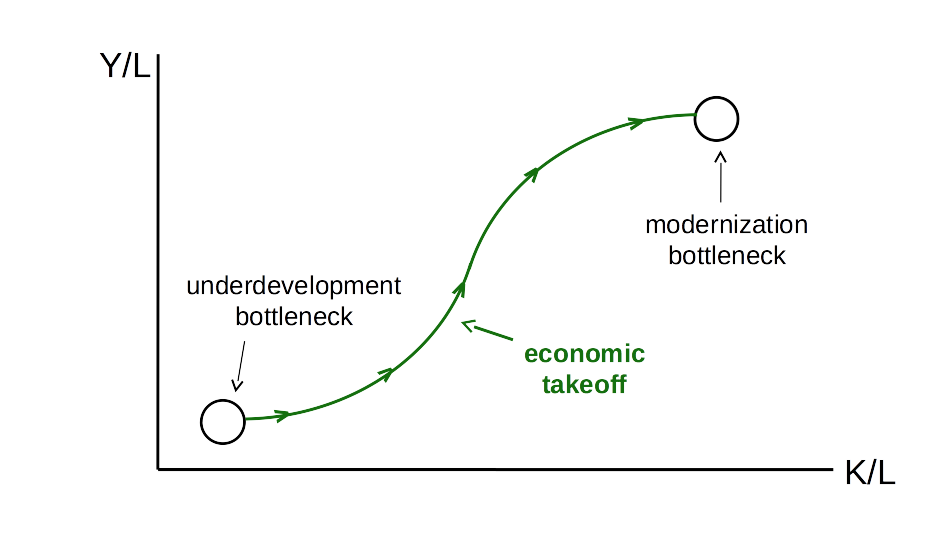
\includegraphics[scale=0.4]{figures/1}
	\caption{图示例}
\end{figure}

\lstinputlisting[caption={test.m}\label{aaa}]{codes/test.m}

	
\lstinputlisting[caption={test.m}\label{lt2}]{codes/test.m}

\ref*{lt1} \ref{lt2}

\section{参考文献例子}

参考文献。\ref{aaa}\cite{jls2003}\cite{Grisvard1985} 

{\bf 参考文献请务必用bibtex生成！！！}\cite{Agnelli2017,Ammari2007}


\chapter{结论}

Enjoy it.
\newline%%紧跟正文最后一个字符的不要删除！



%%%参考文献请务必用bibtex生成！！！
\bibliography{bib/ref.bib}	



\chapterx{致谢}

谢谢。本模板仅供内部使用，谢谢配合。



%\chapterx{个人简历}
%
%
\begin{resume}

\begin{resumesection}{基本情况}
某某某, 男/女, 某某省某某市/县人, 199？/200？ 年~？ 月出生.
\end{resumesection}

\begin{resumelist}{教育状况}
20XX 年~9 月至~20XX 年~7 月, 某某学校某某学院, 本科, 专业: XXXX。

20XX 年~9 月至~201XX年~7 月, 上海财经大学统计与管理学院, 硕士研究生, 专业: XXX。
\end{resumelist}
%
%\begin{resumelist}{工作经历}

%\end{resumelist}

\begin{resumesection}{研究兴趣}
XXXXX。
\end{resumesection}

\begin{resumesection}{联系方式}
E-mail: XXXXX@mail.shufe.edu.cn.
\end{resumesection}
%
\end{resume}




\end{document}
